\section{Metadata: Serialization}

\begin{frame}{Day 2 - Part 4: Metadata Serialisation}{10:00 - 10:45}
    \begin{block}{Module 4 Goal}
        Welcome to Day 2! We will focus on the \textit{structure} and \textit{format} of metadata. It's not just \emph{what} you record, but \emph{how} you encode it.
    \end{block}
    \begin{center}
        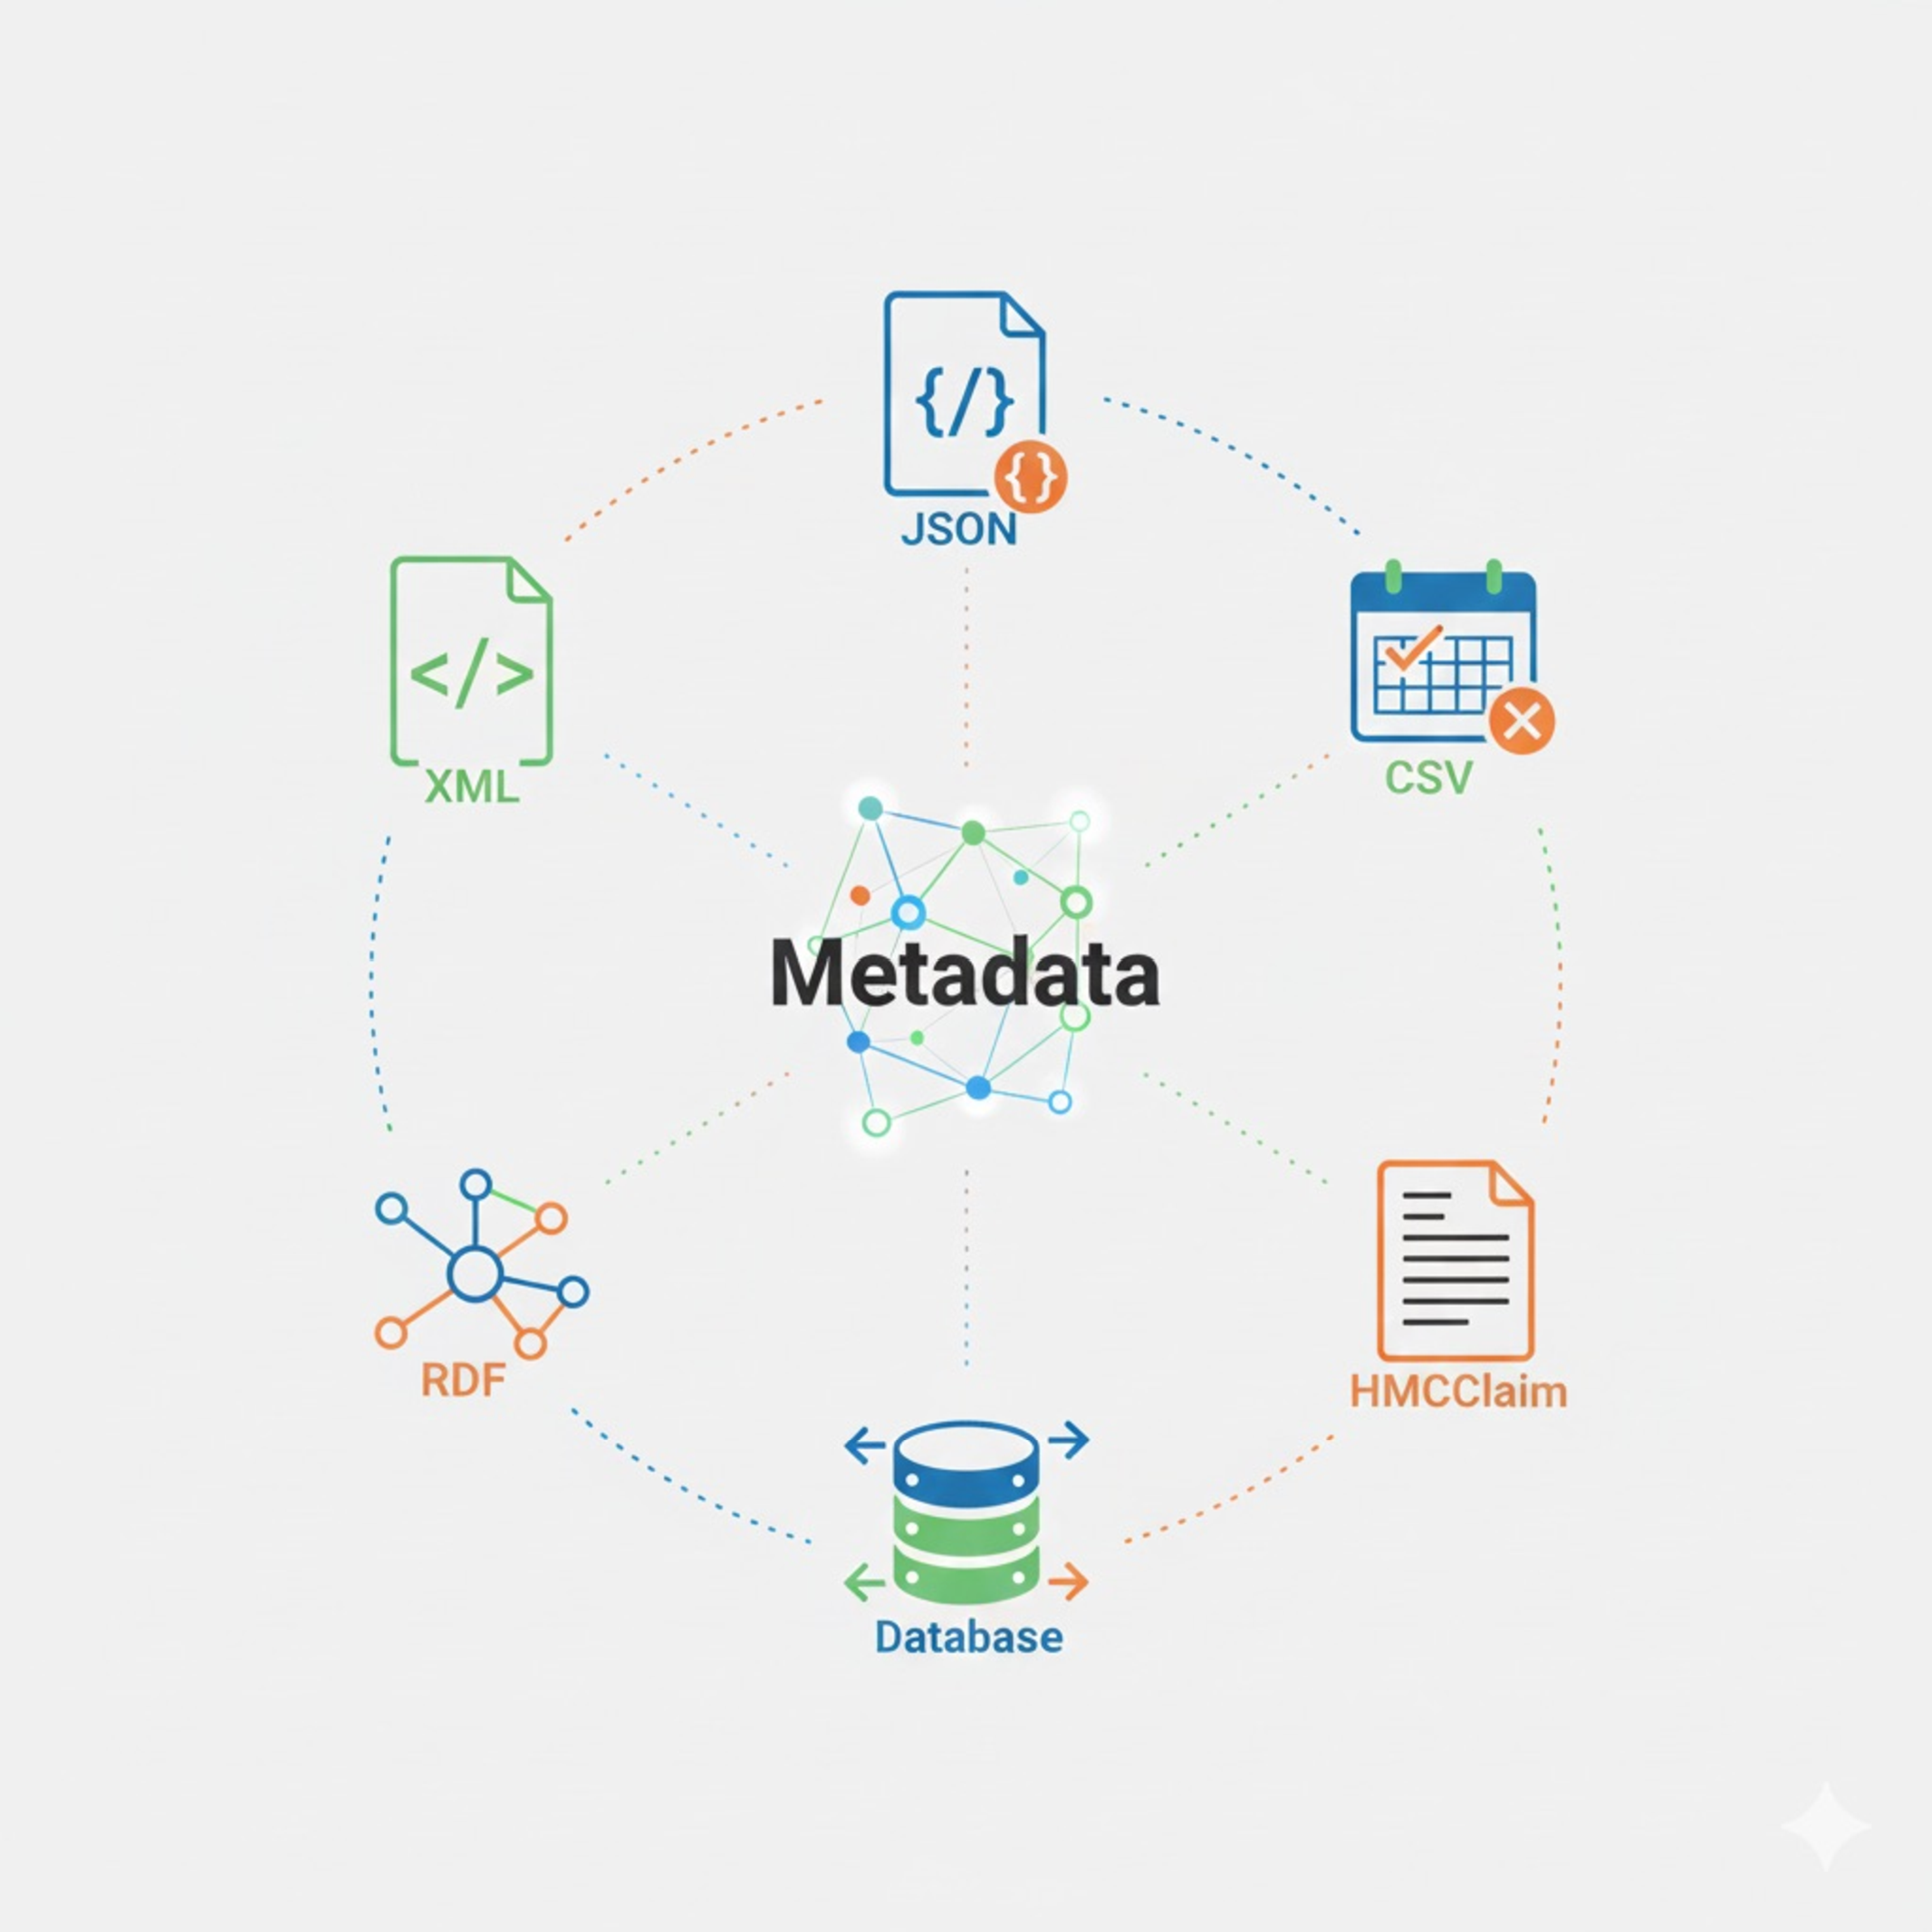
\includegraphics[width=0.32\textwidth]{figs/fig_d2p4/fig_d2p4_01-container}
        \captionof{figure}{Metadata can be stored in many different "containers" (formats).}
    \end{center}
\end{frame}

\begin{frame}{Learning Objectives (4.1)}
    \begin{itemize}
        \item \textbf{Recall} the core components of a minimal metadata standard (e.g., Dublin Core).
        \item \textbf{Recall} the structural differences between common metadata serialisation formats (XML, JSON, CSV).
    \end{itemize}
\end{frame}

\begin{frame}{Theory: Minimal Standard (Dublin Core)}{Module 4.1: Recall}
    \textbf{Dublin Core (DC)} is a "lowest common denominator" metadata standard. It provides 15 simple fields to describe \textit{anything}.
    
    \begin{block}{The 15 Dublin Core Elements}
        \begin{columns}
            \column{.32\textwidth}
            \begin{itemize}
                \item Title
                \item \textbf{Creator}
                \item Subject
                \item \textbf{Description}
                \item Publisher
            \end{itemize}
            
            \column{.32\textwidth}
            \begin{itemize}
                \item Contributor
                \item \textbf{Date}
                \item \textbf{Type}
                \item \textbf{Format}
                \item \textbf{Identifier}
            \end{itemize}
            
            \column{.32\textwidth}
            \begin{itemize}
                \item Source
                \item Language
                \item Relation
                \item Coverage
                \item \textbf{Rights} (License)
            \end{itemize}
        \end{columns}
    \end{block}
    This is the minimum you should provide for 'F' and 'R'.
\end{frame}

\begin{frame}[fragile]{Theory: Serialisation Formats}{Module 4.1: Recall}
    How do we write this metadata down?
    
    \begin{columns}
        \column{.33\textwidth}
        \begin{block}{CSV}
        \vspace{1.2ex}
            \begin{lstlisting}[language=CSV]
Title,Creator
My Data,A. Researcher
            \end{lstlisting}
            \vspace{1.2ex}
            \begin{itemize}
                \item Simple
                \item No hierarchy
            \end{itemize}
            
        \end{block}
        
        \column{.33\textwidth}
        \begin{block}{XML}
        \vspace{1.2ex}
            \begin{lstlisting}[language=XML]
<Title>My Data</Title>
<Creator>A. Researcher</Creator>
            \end{lstlisting}
            \vspace{1.2ex}
            \begin{itemize}
                \item Verbose
                \item Strict (Schemas!)
            \end{itemize}
        \end{block}
        
        \column{.33\textwidth}
        \begin{block}{JSON}
            \begin{lstlisting}[language=json]
{
  "Title": "My Data",
  "Creator": "A. Researcher"
}
            \end{lstlisting}
            \begin{itemize}
                \item Web-friendly
                \item Less strict
            \end{itemize}
        \end{block}
    \end{columns}
\end{frame}

\begin{frame}{Interactive: Format Brainstorm}
    \framesubtitle{Module 4.1: Practice}
    \begin{block}{Group Brainstorm (10 min)}
        \textbf{Task:} Let's \textbf{recall} the pros and cons of these formats.
        \begin{itemize}
            \item When would \textbf{CSV} be a \textit{good} choice for metadata?
            \pause
            \item When would \textbf{XML} be a \textit{better} choice than JSON? (Hint: Think about strict rules).
            \pause
            \item Why has \textbf{JSON} become the most popular format for web APIs?
        \end{itemize}
    \end{block}
\end{frame}

\begin{frame}{Learning Objectives (4.2)}
    \begin{itemize}
        \item \textbf{Differentiate} between \textbf{descriptive} and \textbf{technical} metadata.
        \item \textbf{Differentiate} between the role of a \textbf{metadata schema} (structure) and a \textbf{serialisation format} (encoding).
    \end{itemize}
\end{frame}

\begin{frame}{Theory: Types of Metadata}
    \framesubtitle{Module 4.2: Differentiate}
    Not all metadata is the same.
    
    \begin{columns}
        \column{.5\textwidth}
        \begin{block}{Descriptive Metadata}
            \textbf{What} the data is.
            \begin{itemize}
                \item Title
                \item Creator
                \item Abstract
                \item Keywords
            \end{itemize}
            \textbf{Purpose:} Findability, Citation. ('F', 'R')
        \end{block}
        
        \column{.5\textwidth}
        \begin{block}{Technical Metadata}
            \textbf{How} the data was made.
            \begin{itemize}
                \item `Software: Python 3.9`
                \item `Instrument: HMC-Microscope-047`
                \item `File Format: .csv`
                \item `Checksum: md5:ab...c1`
            \end{itemize}
            \textbf{Purpose:} Reusability, Validation. ('I', 'R')
        \end{block}
    \end{columns}
\end{frame}

\begin{frame}{Theory: Schema vs. Serialisation}
    \framesubtitle{Module 4.2: Differentiate}
    This is the most important concept in this module.
    
    %% \begin{center}
    %%     \includegraphics[width=0.7\textwidth]{example-image-a}
    %% \end{center}
    
    \begin{itemize}
        \item \textbf{Schema (The Blueprint):} The \textit{rules}.
        \item "You MUST have a Title. The Date MUST be in `YYYY-MM-DD` format."
        \item (e.g., Dublin Core, XSD, JSON-Schema)
        \pause
        \item \textbf{Serialisation (The Building Material):} The \textit{format} you write it in.
        \item "We will write these rules in XML."
        \item (e.g., XML, JSON, Turtle)
    \end{itemize}
    \pause
    You can use the \textbf{Dublin Core schema} and serialise it as \textbf{XML}, \textbf{JSON}, or even \textbf{CSV}.
\end{frame}

\begin{frame}{Interactive: Schema or Format?}
    \framesubtitle{Module 4.2: Practice}
    \begin{block}{Quiz (10 min)}
        I'll name a term. You tell me: \textbf{Schema (Rule)} or \textbf{Serialisation (Format)}?
        \pause
        \begin{itemize}
            \item JSON? $\rightarrow$ \textbf{Format}
            \pause
            \item Dublin Core? $\rightarrow$ \textbf{Schema}
            \pause
            \item XML? $\rightarrow$ \textbf{Format}
            \pause
            \item ISO 19115 (for Geospatial data)? $\rightarrow$ \textbf{Schema}
            \pause
            \item `metadata.csv`? $\rightarrow$ \textbf{Format}
            \pause
            \item JSON-Schema? $\rightarrow$ \textbf{Schema} (A schema for the JSON format!)
        \end{itemize}
    \end{block}
\end{frame}

\begin{frame}{Learning Objectives (4.3)}
    \begin{itemize}
        \item \textbf{Annotate} a raw dataset file by applying a selected discipline-specific metadata standard.
        \item \textbf{Annotate} a raw dataset file by applying a minimal metadata schema (Dublin Core) and exporting the result in a serialisation format (JSON).
    \end{itemize}
\end{frame}

\begin{frame}{Theory: What is Annotation?}
    \framesubtitle{Module 4.3: Annotate}
    Annotation is the act of \emph{linking} a piece of data to its metadata.
    
    \begin{block}{Example Annotation}
        \textbf{Raw Data:} `my\_experiment.csv`
        \pause
        \textbf{Annotation (in a separate JSON file):}
% \begin{lstlisting}[language=json]
% {
%   "file_name": "my_experiment.csv",
%   "dc:title": "Temperature Experiment",
%   "dc:creator": "Researcher, A.",
%   "dc:date": "2025-11-14",
%   "my_schema:instrument": "HMC-Microscope-047"
% }
% \end{lstlisting}
    \end{block}
    \pause
    This file now describes the raw data. This is a \textbf{Metadata Record}.
\end{frame}

\begin{frame}{Interactive: Let's Annotate!}
    \framesubtitle{Module 4.3: Practice}
    \begin{block}{Workshop: Annotate a File (20 min)}
        \textbf{Task:} Everyone take a simple file on your computer (a script, a CSV, a document).
        \pause
        \begin{enumerate}
            \item Open a plain text editor (e.g., Notepad, VS Code).
            \item Create a new file called `metadata.json`.
            \item \textbf{Annotate} your file using \textbf{Dublin Core} (Title, Creator, Date, Format).
            \item Write this annotation in \textbf{JSON format} (like the previous slide).
        \end{enumerate}
        \pause
        \textbf{Bonus:} Add one \textbf{discipline-specific} field (e.g., `my\_field:sample\_type`). \\
        \pause
        \textbf{Goal:} \textbf{Annotate} a file and \textbf{export} to JSON.
    \end{block}
\end{frame}

\begin{frame}{Learning Objectives (4.4)}
    \begin{itemize}
        \item \textbf{Compare} two different metadata files (XML vs. JSON) and \textbf{analyse} their efficiencies (machine readability, schema validation).
        \item \textbf{Compare} two different serialisation formats (XML vs. JSON) and \textbf{analyse} their efficiencies (parsing overhead).
    \end{itemize}
\end{frame}

\begin{frame}{Theory: Comparing XML vs. JSON}
    \framesubtitle{Module 4.4: Compare}
    \begin{columns}
        \column{.5\textwidth}
        \begin{block}{XML (eXtensible Markup Language)}
% \begin{lstlisting}[language=XML]
% <root>
%   <dc:title>My Data</dc:title>
%   <dc:creator>A. Researcher</dc:creator>
% </root>
% \end{lstlisting}
            \begin{itemize}
                \item \textbf{Pro:} Very strict validation using XSD (XML Schema).
                \item \textbf{Pro:} Supports Namespaces (e.g., `dc:`).
                \item \textbf{Con:} "Verbose" (high parsing overhead).
            \end{itemize}
        \end{block}
        
        \column{.5\textwidth}
        \begin{block}{JSON (JavaScript Object Notation)}
% \begin{lstlisting}[language=json]
% {
%   "@context": {"dc": "..."},
%   "dc:title": "My Data",
%   "dc:creator": "A. Researcher"
% }
% \end{lstlisting}
            \begin{itemize}
                \item \textbf{Pro:} Lightweight (low parsing overhead).
                \item \textbf{Pro:} Native to web browsers.
                \vspace{3.2ex}
                \item \textbf{Con:} Validation (JSON-Schema) is less mature than XSD.
            \end{itemize}
            
        \end{block}
    \end{columns}
\end{frame}

\begin{frame}{Concept: Readability vs. Validation}
    \framesubtitle{Module 4.4: Analyse}
    \begin{itemize}
        \item \textbf{Machine Readability / Parsing Overhead:}
        \item JSON is "lighter" and faster for a web browser to parse. This is why it's used for web APIs.
        \pause
        \item \textbf{Schema Validation:}
        \item XML is "stricter." It's often preferred by archives and large institutions (like libraries) because an XSD schema can enforce very complex rules, guaranteeing metadata integrity.
    \end{itemize}
    \pause
    \begin{block}{Which is "better"?}
        Neither. They are different tools.
        \begin{itemize}
            \item Use \textbf{JSON} for fast, lightweight data exchange (e.g., web pipelines).
            \item Use \textbf{XML} for strict, archival-grade metadata validation.
        \end{itemize}
    \end{block}
\end{frame}

\begin{frame}{Interactive: Which is "Better"?}
    \framesubtitle{Module 4.4: Practice}
    \begin{block}{Discussion (10 min)}
        Let's \textbf{compare} and \textbf{analyse}.
        \pause
        \begin{itemize}
            \item \textbf{Scenario 1:} You are building a web dashboard to show live sensor data. Which format do you use?
            \item \emph{Answer:} JSON (low overhead).
            \pause
            \item \textbf{Scenario 2:} You are submitting your final metadata to a 100-year archive (like the national library). Which format do they probably want?
            \item \emph{Answer:} XML (strict validation).
        \end{itemize}
    \end{block}
\end{frame}

\begin{frame}{Learning Objectives (4.5)}
    \begin{itemize}
        \item \textbf{Justify} the selection of a specific \textbf{controlled vocabulary} to transform free-text into standardised terms.
        \item \textbf{Justify} the selection of a specific \textbf{serialisation format} for a project based on pipeline constraints.
    \end{itemize}
\end{frame}

\begin{frame}{Theory: The Problem with Free-Text}{Module 4.5: Justify}
   %% \begin{center}
   %%     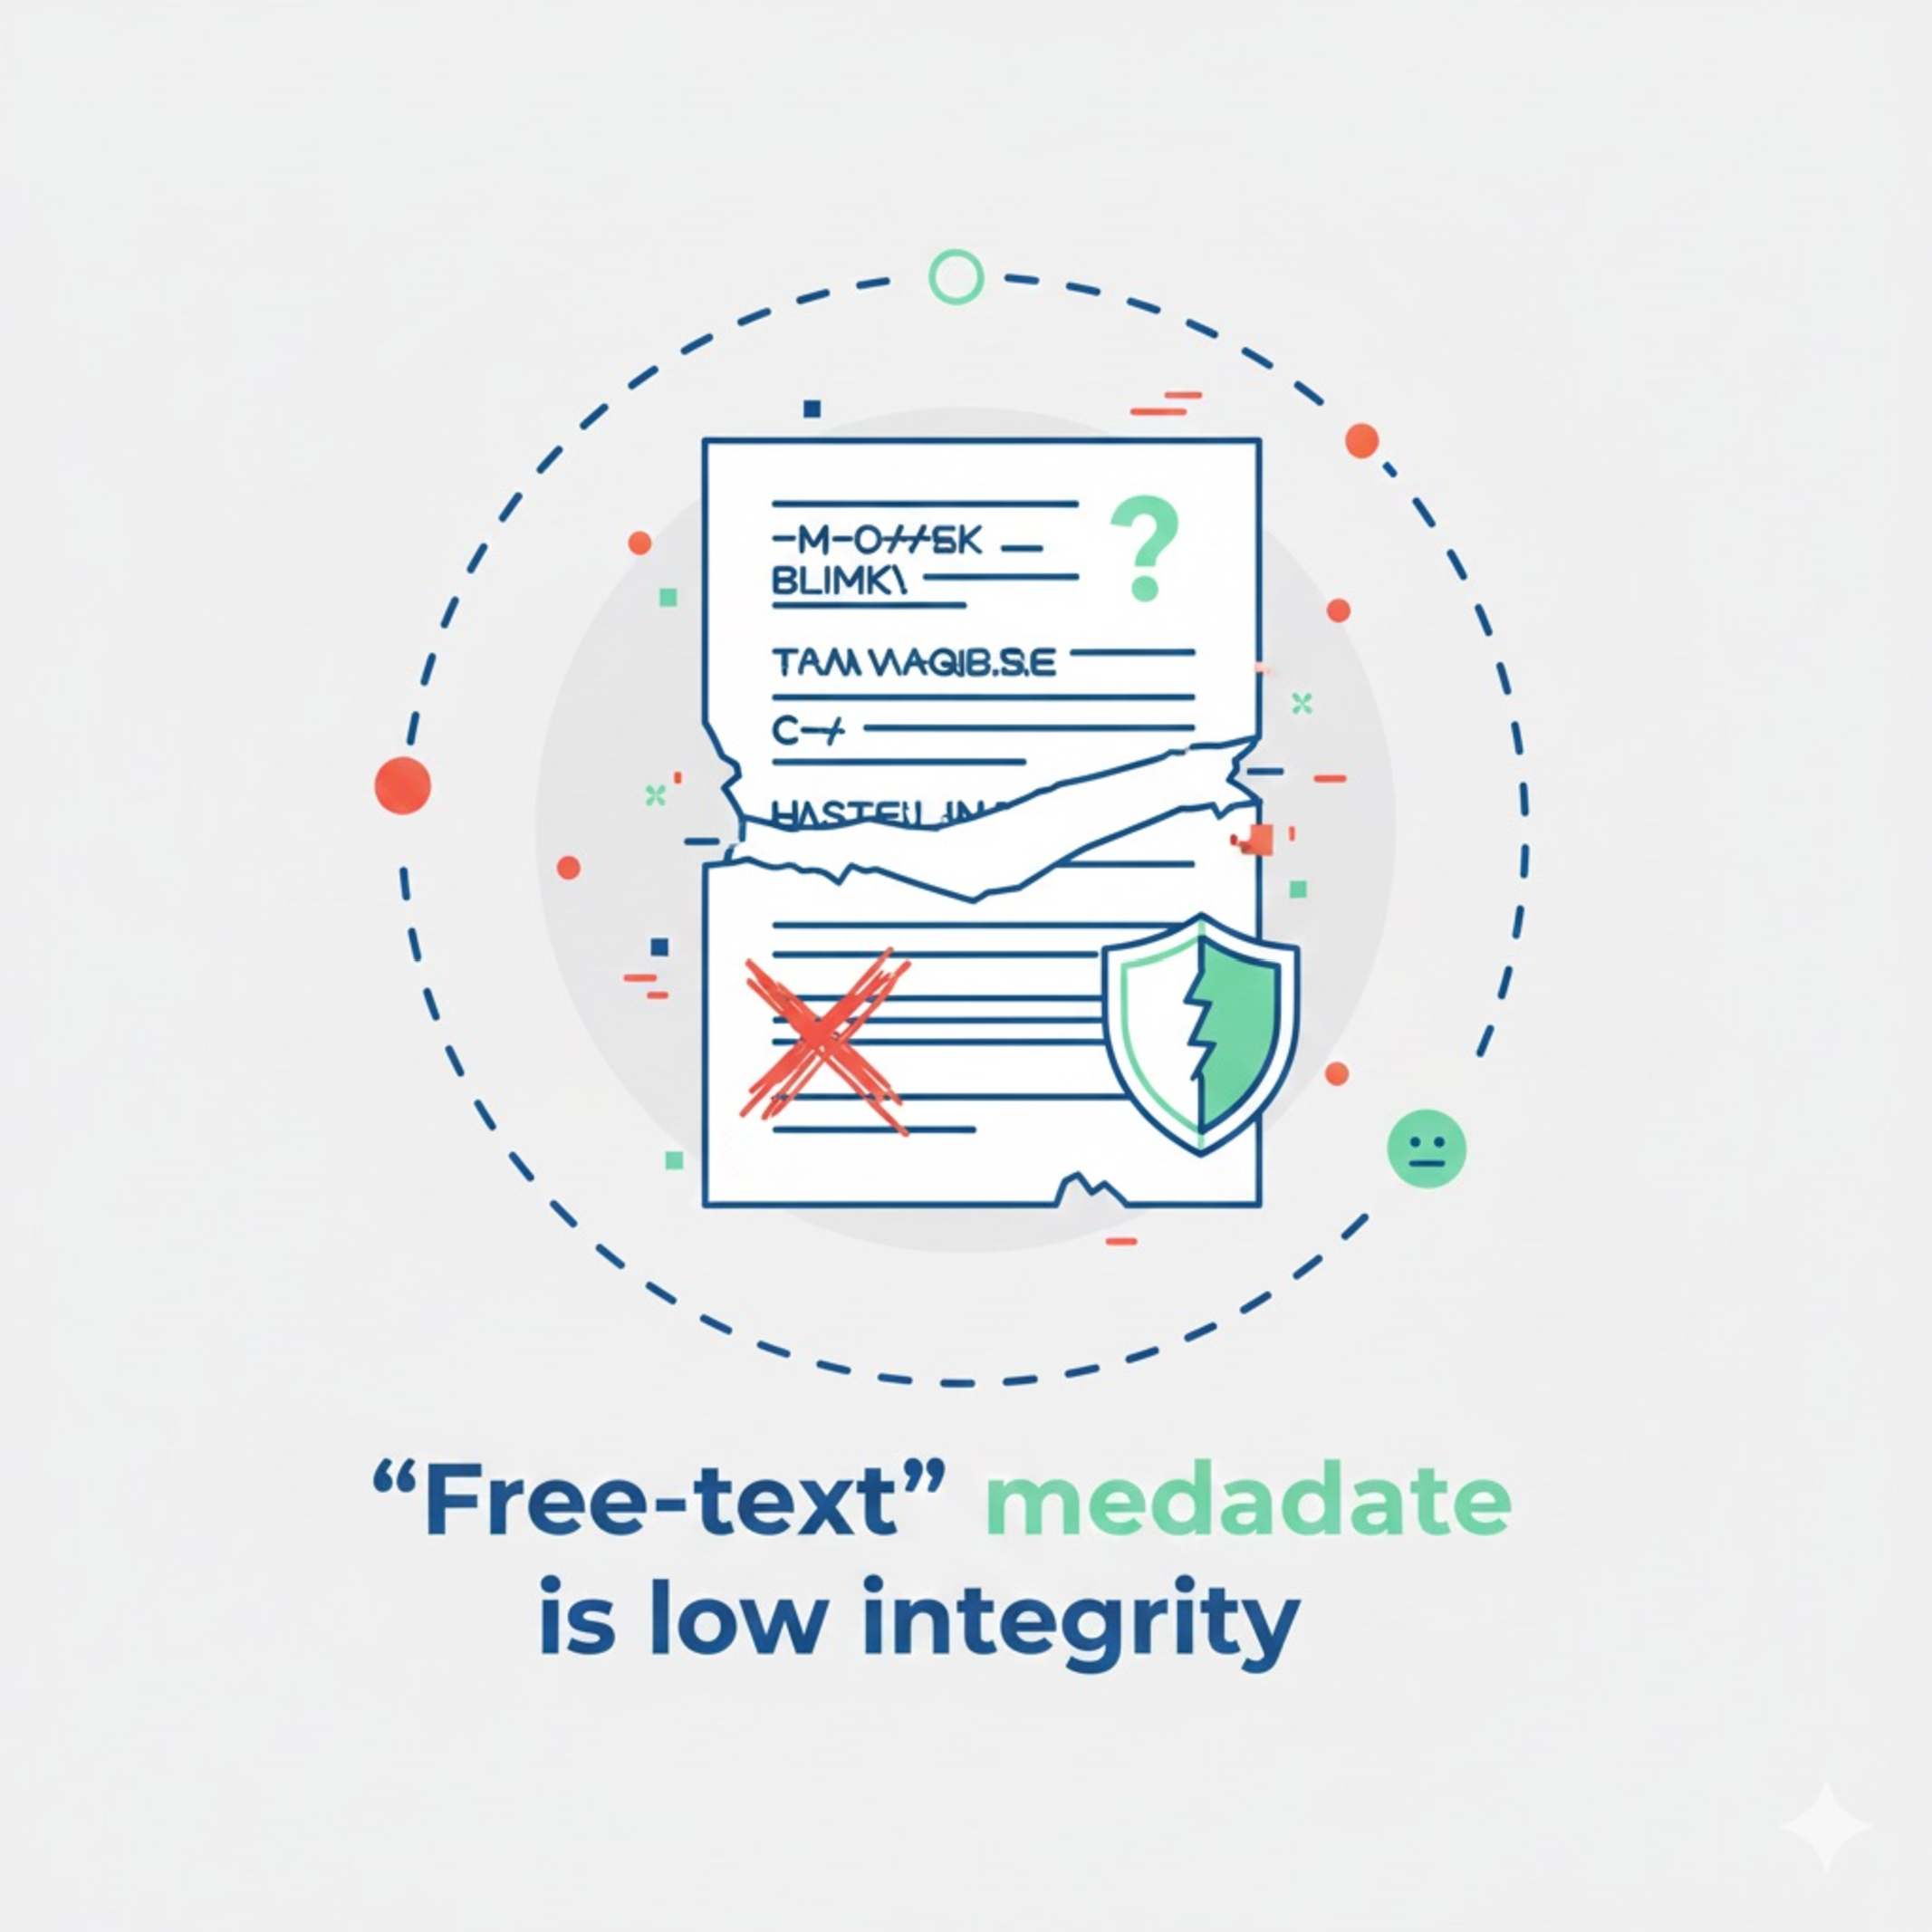
\includegraphics[width=0.32\textwidth]{figs/fig_d2p4/fig_d2p4_02-freetext}
   %%     \captionof{figure}{"Free-text" metadata is low integrity.}
   %% \end{center}
   \begin{columns}
       \column{.4\textwidth}
    \begin{block}{A "Free-Text" Metadata Record}
        \begin{itemize}
            \item `Location: Karlsruhe`
            \item `Location: KIT Campus North`
            \item `Location: 76131, Germany`
        \end{itemize}
    \end{block}
    \pause
    \column{.6\textwidth}
    A machine \textbf{cannot} understand that these are the same place. The data is not Interoperable ('I').\\
    \pause
    \textbf{Solution:} Transform free-text using a \textbf{Controlled Vocabulary (CV)}.
    \pause
    \begin{block}{A "Standardised" Metadata Record}
        \begin{itemize}
            \item `Location: https://geonames.org/2892794` (URI for Karlsruhe)
        \end{itemize}
    \end{block}
    Now, a machine knows \textit{exactly} where you mean.
   \end{columns}
\end{frame}

\begin{frame}{Interactive: The Pipeline Choice}
    \framesubtitle{Module 4.5: Practice}
    \begin{block}{Scenario (15 min)}
        \textbf{Situation:} Your data pipeline must feed two systems:
        \begin{enumerate}
            \item A web dashboard (needs to be fast).
            \item A long-term HMC archive (needs to be strict).
        \end{enumerate}
        \pause
        \textbf{Task:}
        \begin{itemize}
            \item \textbf{Justify} the \textbf{serialisation format} you would choose for \#1. (JSON)
            \pause
            \item \textbf{Justify} the \textbf{serialisation format} you would choose for \#2. (XML)
            \pause
            \item How do you serve both? (Answer: You don't pick one. You \emph{transform} your internal data \textit{into} both formats!)
        \end{itemize}
    \end{block}
\end{frame}

\begin{frame}{Learning Objectives (4.6)}
    \begin{itemize}
        \item \textbf{Transform} a project's internal, proprietary metadata scheme into an \textbf{interoperable} format (e.g., XSLT).
        \item \textbf{Transform} a project's internal, proprietary metadata scheme into a \textbf{standardized serialization format}.
    \end{itemize}
\end{frame}

\begin{frame}{Theory: Metadata Transformation}
    \framesubtitle{Module 4.6: Transform}
    You will almost \textit{never} work in the final format. You work in what's easy (your ELN, a CSV), and then \textbf{transform} it for publication.
    
    %% \begin{center}
    %%     \includegraphics[width=0.8\textwidth]{example-image-c}
    %%     \captionof{figure}{Your Internal CSV $\rightarrow$ Transformation Script $\rightarrow$ XML, JSON, etc.}
    %% \end{center}
    
    \begin{block}{Common Transformation Tools}
        \begin{itemize}
            \item \textbf{XSLT:} A language specifically for transforming XML $\rightarrow$ XML or XML $\rightarrow$ HTML.
            \item \textbf{Python/R Script:} The most common. Read a CSV/JSON, use a library to write out a valid XML file.
            \item \textbf{LinkML:} (See next module) Can auto-generate transformers.
        \end{itemize}
    \end{block}
\end{frame}

\begin{frame}{Interactive: Transformation Needs}
    \framesubtitle{Module 4.6: Practice}
    \begin{block}{Discussion (10 min)}
        \textbf{Task:} Let's think about your own research.
        \begin{itemize}
            \item What is your \textbf{internal, proprietary} format? (e.g., "The `.dat` file from my instrument," "My personal Excel template.")
            \pause
            \item What is the \textbf{standardised format} your field or repository wants? (e.g., "The OEP wants standards-compliant metadata.")
            \pause
            \item What is the "transformation" gap you need to bridge?
        \end{itemize}
        \pause
        \textbf{Goal:} \textbf{Transform} (conceptually) your internal format to a standard one.
    \end{block}
\end{frame}

\begin{frame}{Module 4: Summary}
    \begin{itemize}
        \item \textbf{Metadata} has many types (Descriptive, Technical).
        \item \textbf{Schema} (the rules) and \textbf{Serialisation} (the format) are different.
        \item \textbf{XML} is for validation; \textbf{JSON} is for web-friendliness.
        \item We must \textbf{transform} our internal, free-text metadata into \textbf{standardised, vocabulary-controlled} records for publication.
    \end{itemize}
    \vfill
    \begin{center}
        \textbf{End of Part 4}
    \end{center}
\end{frame}